\scanpage{281}
% archive sheet number: 280

\[
\left\{\begin{aligned}
1)\quad &\{\deleted{\unsure{x}}s,\deleted{\unsure{y}}t\}\in A_{\unsure{q|0}},\ \deleted{\unsure{u\in S}}\quad\Longrightarrow\quad
\deleted{\exists}\ \text{il existe exactement deux}\\
&\hspace{14em}\text{éléments }\deleted{\unsure{2u}}\ \text{tels que}\\
&\hspace{14em}\{\deleted{\unsure{x}}s,u\}\ \text{et }\{\deleted{\unsure{y}}t,u\}\in A_0\\
&\deleted{\unsure{\{x,y|\{s,t\}}}\\
2)\quad &\forall\,\deleted{\unsure{x}}s,\deleted{\unsure{y}}t\in S,\ \exists\,u\in S\ \text{tel que}\quad\{s,u\},\{t,u\}\in A\\
&\hspace{8em}\text{et OPS }\{s,u\}\in A_0
\end{aligned}\right.
\]

\deleted{\uline{Corollaire}}\qquad \uline{Corollaire} $\forall\,s,t\in S$, $\exists\,u,v,w\in S$ tels que $(s,u,v,\deleted{\unsure{w}},t)$ soit une $A_0$ chaine.

\diagram{\begin{tikzcd}[ampersand replacement=\&,column sep=small,row sep=small]
s\arrow[dr,no head,"0"'] \& \& \& t\\
\& u\arrow[r,no head,"0"]\arrow[dr,no head,"\deleted{\unsure{0}}"'] \& \unsure{v|w}\arrow[ur,no head,"0"']\arrow[dl,no head,"{\deleted{\unsure{0}}}"] \&\\
\&\&\deleted{\unsure{w|v}}\&
\end{tikzcd}}

\uline{Dém} Par 2) \inserted{pour $(s,t)$} on choisit $u$ avec

\[
\begin{aligned}
&\{s,u\}\in A_0\\
&\{u,t\}\in A
\end{aligned}
\]

puis par 1) pour $(u,t)$, on choisit $v$ qui relie $u$ à $t$ par $A_0$

\[
\underline{3)\quad A(s)=A(t)}\quad\Longrightarrow\quad\exists(u,v)\in S^2,
\]

\diagram{\begin{tikzcd}[ampersand replacement=\&,column sep=small,row sep=tiny]
\&s\arrow[dr,no head,"0"]\&\\
u\arrow[ur,no head,"0"]\arrow[rr,no head,"A" description]\arrow[dr,no head,"A"']\&\& v\\
\&t\arrow[ur,no head,"A"']\&
\end{tikzcd}\quad$|\!|\!|$}

\uwave{Sommet déterminé par son étoile} ?

Pas vrai pour $\Lambda=\mathbb Z/4\mathbb Z$ (octaèdre) car deux éléments de $M^*$, savoir $u$ et \deleted{\unsure{$u+2v$}} $\underline a\,u$

\deleted{$=u+2\unsure{w}$ \unsure{ou} $u+2u$ \unsure{ou|$=3u=$} $u+2v$ ($v$} \deleted{$u'=u$}\ \deleted{\unsure{$\operatorname{Et}\ M_u^*=$|$\operatorname{Et}\ M_2^*=$}}

\[
\begin{aligned}
&x\wedge u=\pm x'\wedge u\qquad\text{quand}\\
&x\wedge u\ \text{et }x'\wedge u\ \text{sont }\in\Lambda^*
\end{aligned}
\]

\figure{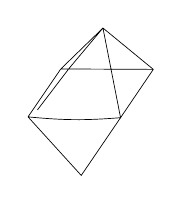
\begin{tikzpicture}[x=.52cm,y=.52cm,line width=.25pt]
\coordinate (a) at (0,0);\coordinate (b) at (1.30,-1.43);\coordinate (c) at (2.26,-.02);
\coordinate (d) at (3.06,1.16);\coordinate (e) at (1.83,2.17);\coordinate (f) at (.80,1.17);
\draw (a)--(b)--(c)--(d) (a)--(f)--(e)--(d) (a) to[bend right=5] (c) (e)--(c)
(f)--(d) (.23,.17)--(1.00,1.18)--(e);
\end{tikzpicture}}

\[
\begin{aligned}
x,\deleted{x'}&=\lambda e+\mu f & x\wedge e&=\pm\mu & x\wedge f&=\pm\lambda\\
x'&=\lambda'e+\mu'f & x'\wedge e&=\pm\mu' & x'\wedge f&=\pm\lambda'\\
\deleted{x\wedge}\ u&=ae+bf & \text{ops}\quad x&=e+\deleted{\unsure{f}}f & u&=\unsure{\checkmark}\\
&&x'&=e-f\\
x\wedge u&=-a+b &\deleted{\unsure{-a+b|a+b}}\\
x'\wedge u&=+a+b & 2a&=0\quad\underline{\text{ou}}\quad 2b=0 &
\deleted{\underline{\text{si }(a,b)=\Lambda}},\quad b-a,\ b+a&\in\Lambda^*
\end{aligned}
\]
